\newcommand{\req}[1]{RQ#1}
\begin{table*}[t]
  \vspace{2mm}
  \caption{The analysis result of NativeFlowBench}
  \label{table:RQ1}
  \vspace*{-1em}
  \centering
  \small
  \begin{tabular}{l|c|c|c|c||l|c|c|c|c}
    \myhead{Benchmark}{Precision}{Dataflow}
    %\myhead{Benchmark}{Lee~\cite{LeeASE20}}{Ours}{Benchmark}{JN-SAF}{Ours}
    icc\_javatonative                   & X & X & O & X & native\_noleak                       & O & O & O & O  \\
    icc\_nativetojava                   & O & O & O & X & native\_noleak\_array                & O & O & X & O  \\
    native\_complexdata                 & O & O & O & O & native\_nosource                     & O & O & O & O  \\
    native\_complexdata\_stringop       & X & X & X & X & native\_pure                         & X & O & O & O  \\
    native\_dynamic\_register\_multiple & O & O & O & O & native\_pure\_direct                 & X & O & O & O  \\
    native\_heap\_modify                & O & O & O & O & native\_pure\_direct\_customized     & X & O & O & O  \\
    native\_leak                        & O & O & O & O & native\_set\_field\_from\_arg        & O & O & O & O  \\
    native\_leak\_array                 & O & O & O & X & native\_set\_field\_from\_arg\_field & O & O & O & O  \\
    native\_leak\_dynamic\_register     & O & O & O & O & native\_set\_field\_from\_native     & O & O & O & O  \\
    native\_method\_overloading         & O & O & O & O & native\_source                       & O & O & O & O  \\
    native\_multiple\_interactions      & O & O & O & O & native\_source\_clean                & O & O & O & O  \\
    native\_multiple\_libraries         & O & O & O & O & \multicolumn{1}{c}{}                 & \multicolumn{1}{c}{} & \multicolumn{1}{c}{} & \multicolumn{1}{c}{} & \multicolumn{1}{c}{}
  \end{tabular}
\end{table*}



\section{Evaluation}\label{sec:eval}

To show the effectiveness of our approach, we evaluate our analyzer
JN-QL with the following three research questions:
\begin{itemize}
  \item \textbf{\req{1}: Feasibility.} Can \ours analyze JNI programs that use
    various JNI inteoperations?

  \item \textbf{\req{2}: Performance.} How precise and scalable is \ours for
    real-world JNI program analysis compared to JN-Sum~\cite{LeeASE20}?

  \item \textbf{\req{3}: Usefulness.} Can \ours analyze the same kinds of bugs
    the state-of-the-art JNI program analyzers can detect?
\end{itemize}

For \req{1}, we analyze the benchmarks in NativeFlowBench~\cite{nativeflowbench,
JN-SAF} using \ours. The benchmarks contain 23 JNI Android applications (apps) that
use various JNI interoperations and sensitive data leakage from {\it sources} to
{\it sinks} across language boundaries via the interoperations. We compare
the analysis results of \ours to the results of JN-Sum and JN-SAF. We use
compiled versions of the benchmarks for JN-SAF because it targets compiled JNI
programs and uses the source code of the benchmarks for \ours and JN-Sum.

For \req{2}, we compare the analysis results of \ours and JN-Sum on 42
real-world JNI Android apps downloaded from F-Droid, a repository of
open-source Android apps~\cite{fdroid}. We first classified
F-Droid apps into JNI and non-JNI apps. Then, we selected
all 42 apps that can be compiled without any errors as our analysis targets.

For \req{3}, we detect JNI interoperation bugs in the 42 real-world Android
apps using \ours. We implemented a checker detecting four kinds of
bugs on top of \ours using the query language of CodeQL. We chose our target
JNI interoperation bugs as the same as the targets of the client
analysis of the previous research~\cite{LeeASE20, ILEA}.


\subsection{\req{1}: Feasibility}
Table~\ref{table:RQ1} summarizes the analysis results of \ours, JN-Sum,
and \jnsaf on 23 benchmarks in NativeFlowBench.
The {\bf Benchmark} columns show the benchmark names,
{\bf Precision} show the analysis results of 
JN-Sum and \ours, and {\bf Dataflow} show the analysis results of JN-SAF and \ours.
JN-Sum and JN-SAF have different analysis purposes from
each other; JN-Sum constructs call graphs of JNI programs, and JN-SAF
detects data leakages from sources to sinks.  For fair comparison, we compare
\ours and JN-Sum for the precision of resolving targets of foreign
function calls, and compare \ours and JN-SAF for the data leakage detection results.
We marked each analysis result as a success ($\bigcirc$) or failure ($\times$).
In the precision comparison, an analysis succeeds if
it precisely resolves targets of all foreign function calls between Java and C, and it fails otherwise.
In the dataflow comparison, an analysis succeeds
if it reports all data leakages correctly without any false positives or negatives.


In the precision comparison, \ours successfully analyzed 21 out of 23
benchmarks, while JN-Sum failed in three more benchmarks than \ours.
We manually confirmed that the two failures both in \lees and \ours
come from built-in structs and functions in C; {\it
icc\_javatonative} stores Java class information in the Android built-in
struct {\tt android\_app} and {\it native\_complexdata\_stringop} generates
a Java field name by concatenating two string values via the {\tt strcat} built-in function.
  Because \ours and JN-Sum do not handle such built-in
structs and functions, they failed to analyze the two benchmarks.
  \lees failed to analyze three more benchmarks due to native entry points
of the benchmarks~\cite{nativeactivity}.
  FlowDroid~\cite{Flowdroid} used by JN-Sum performs a whole-program
analysis from Android entry points. 
  Because the benchmarks have entry points only in C differently from monolingual
Android apps, FlowDroid cannot find entries from which its analysis starts.
  Contrary to JN-Sum, \ours performs a query-based
analysis, which can resolve the targets of foreign function calls regardless of program entries.

\begin{table*}[t]
  \vspace{2mm}
  \caption{The analysis result for F-Droid applications}
  \label{table:RQ2}
  \vspace*{-1em}
  \centering
  \small
  \begin{tabular}{l||r|r|r|r|r||r|r|r||r|r|r}
    \multirow{3}{*}{\textbf{Application}} & \multicolumn{5}{c||}{\textbf{Time (sec.)}} & \multicolumn{3}{c||}{\multirow{2}{*}{\textbf{C->Java Function Call}}} & \multicolumn{3}{c}{\multirow{2}{*}{\textbf{C->Java Field Access}}} \\\hhline{~||-----||~~~||~~~}
    & \multicolumn{3}{c|}{\textbf{DB Creation}} & \multicolumn{1}{c|}{\multirow{2}{*}{\textbf{Query}}} & \multicolumn{1}{c||}{\multirow{2}{*}{\textbf{Total}}} & \multicolumn{3}{c||}{} & \multicolumn{3}{c}{} \\\hhline{~||---~|~||------}
    & \multicolumn{1}{c|}{\textbf{C}} & \multicolumn{1}{c|}{\textbf{Java}} & \multicolumn{1}{c|}{\textbf{Merged}} & \multicolumn{1}{c|}{} & \multicolumn{1}{c||}{} & \multicolumn{1}{c|}{\textbf{\# Precise}} & \multicolumn{1}{c|}{\textbf{\# Resolved}} & \multicolumn{1}{c||}{\textbf{Total}} & \multicolumn{1}{c|}{\textbf{\# Precise}} & \multicolumn{1}{c|}{\textbf{\# Resolved}} & \multicolumn{1}{l}{\textbf{Total}}  \\\hhline{=#*{4}{=|}=#=|=|=#=|=|=}
  Agram                  & 2.538                 & 5.002                    & 3.643                      & 6.829                                      & 18.012                                  & 0                           & 0                            & 2                         & 4                           & 4                            & 4                          \\
  AndIodine              & 2.805                 & 8.237                    & 3.989                      & 8.114                                      & 23.145                                  & 1                           & 1                            & 1                         & 0                           & 0                            & 0                          \\
  APV PDF Viewer         & 56.496                & 9.252                    & 23.349                     & 35.688                                     & 124.785                                 & 4                           & 4                            & 4                         & 15                          & 15                           & 16                         \\
  CommonsLab             & 23.176                & 24.139                   & 14.149                     & 20.554                                     & 82.018                                  & 4                           & 5                            & 5                         & 0                           & 0                            & 0                          \\
  CrossWords             & 29.754                & 21.663                   & 23.276                     & 29.106                                     & 103.799                                 & 68                          & 68                           & 70                        & 9                           & 10                           & 14                         \\
  Document Viewer        & 180.71                & 20.292                   & 56.743                     & 75.934                                     & 333.679                                 & 6                           & 6                            & 6                         & 23                          & 23                           & 24                         \\
  DroidZebra             & 17.774                & 7.141                    & 5.817                      & 12.608                                     & 43.34                                   & 4                           & 5                            & 5                         & 0                           & 0                            & 0                          \\
  FBReader               & 85.398                & 27.114                   & 36.36                      & 30.072                                     & 178.944                                 & 0                           & 0                            & 0                         & 0                           & 0                            & 1                          \\
  Fwknop2                & 11.834                & 11.488                   & 7.395                      & 10.446                                     & 41.163                                  & 0                           & 0                            & 0                         & 0                           & 13                           & 13                         \\
  Graph 89               & 72.609                & 8.47                     & 41.465                     & 598.645                                    & 721.189                                 & 1                           & 1                            & 1                         & 0                           & 0                            & 0                          \\
  Irssi ConnectBot       & 1.284                 & 12.32                    & 6.048                      & 11.196                                     & 30.848                                  & 1                           & 1                            & 1                         & 0                           & 0                            & 2                          \\
  Lumicall               & 40.486                & 13.102                   & 17.328                     & 27.104                                     & 98.02                                   & 4                           & 4                            & 4                         & 2                           & 2                            & 13                         \\
  Navit                  & 26.761                & 17.741                   & 54.751                     & 46.264                                     & 145.517                                 & 16                          & 22                           & 55                        & 0                           & 0                            & 0                          \\
  NetGuard               & 14.958                & 16.925                   & 9.988                      & 12.716                                     & 54.587                                  & 0                           & 9                            & 9                         & 3                           & 27                           & 27                         \\
  Overchan               & 1.727                 & 22.043                   & 8.772                      & 15.143                                     & 47.685                                  & 1                           & 2                            & 4                         & 0                           & 0                            & 1                          \\
  Plumble                & 28.501                & 12.365                   & 16.335                     & 29.253                                     & 86.454                                  & 0                           & 0                            & 0                         & 610                         & 610                          & 610                        \\
  PrBoom                 & 48.312                & 5.469                    & 21.601                     & 32.001                                     & 107.383                                 & 7                           & 7                            & 15                        & 0                           & 0                            & 0                          \\
  Rtl-sdr driver         & 18.797                & 16.984                   & 9.623                      & 11.751                                     & 57.155                                  & 2                           & 2                            & 2                         & 0                           & 0                            & 0                          \\
  Sipdroid               & 20.267                & 11.864                   & 10.961                     & 18.577                                     & 61.669                                  & 2                           & 2                            & 2                         & 2                           & 2                            & 16                         \\
  Son of Hunky Punk      & 40.266                & 14.947                   & 20.582                     & 31.102                                     & 106.897                                 & 50                          & 50                           & 52                        & 10                          & 10                           & 10                         \\
  Taps Of Fire           & 3.566                 & 7.521                    & 4.453                      & 8.145                                      & 23.685                                  & 0                           & 0                            & 0                         & 2                           & 2                            & 2                          \\
  Tileless Map           & 273.993               & 187.099                  & 118.557                    & 146.806                                    & 726.455                                 & 50                          & 58                           & 59                        & 3                           & 4                            & 5                          \\
  Timidity AE            & 23.417                & 11.718                   & 13.03                      & 28.452                                     & 76.617                                  & 16                          & 16                           & 16                        & 0                           & 0                            & 0                          \\
  Tux Paint              & 256.126               & 120.831                  & 161.906                    & 184.591                                    & 723.454                                 & 80                          & 83                           & 89                        & 4                           & 4                            & 6                          \\
  VotAR                  & 1.515                 & 5.189                    & 3.569                      & 6.532                                      & 16.805                                  & 1                           & 1                            & 2                         & 3                           & 3                            & 3                          \\\hhline{=#*{4}{=}=#=|=|=#=|=|=}
    \textbf{Total}       & \multicolumn{1}{r}{}  & \multicolumn{1}{r}{}     & \multicolumn{1}{r}{}       & \multicolumn{1}{r}{}                       & \multicolumn{1}{r||}{}                    & 318                         & 347                          & 404                       & 690                         & 729                          & 767
  \end{tabular}
\end{table*}


In the dataflow comparison, \ours found data leakages correctly in 20
benchmarks but reported false negatives for three benchmarks, while JN-SAF
analyzes 21 benchmarks correctly. 
The one common failure comes from string concatenation, as we discussed.
{\it icc\_javatonative} and {\it icc\_nativetojava} leak data via the Android
inter-component communication that is beyond the scope of \ours.
The remaining two different failures of \ours and JN-SAF come from their array analysis policies.
{\it native\_leak\_array} stores sensitive data in an array, retrieves the data from the array,
and leaks it.  On the other hand, {\it native\_noleak\_array} stores sensitive
data in an array as well, but it retrieves another element from the array and uses it.
Because distinguishing different indices of an array is challenging, JN-SAF
tracks every value retrieved from an array if the array contains sensitive data.
Such over-approximation enables JN-SAF to analyze {\it
native\_leak\_array} correctly but introduces a false alarm for {\it
native\_noleak\_array}.  In contrast, because CodeQL does not
track dataflows on arrays by default, \ours does not report
a false alarm for {\it native\_noleak\_array} but cannot find the data leakage in {\it
native\_leak\_array}.


\subsection{RQ2: Performance}
Table~\ref{table:RQ2} summarizes the analysis results of \ours on real-world Android JNI apps.
Out of 42 apps we analyzed, we show the analysis
results of 25 apps that have interoperations from C to Java\footnote{We
report the full analysis results in our supplementary material.}.
The first column shows app names, the second to the fourth columns show database
creation time of C, Java, and their merged database, respectively, the fifth
shows query processing time, and the sixth shows the total analysis time.
{\bf C->Java Function Call} and {\bf C->Java Field Access}
show the numbers of C-to-Java function calls and
C-to-Java field accesses, respectively. We collectively call them
\emph{JNI uses}.
The sub-columns {\bf \#Precise}, {\bf \#Resolved}, and {\bf Total}
represent the numbers of precisely resolved, 
resolved, and the total JNI uses, respectively.
We considered a resolved JNI use as precise, when \ours finds a single target method
or a single field at the JNI use.


\ours resolved 1,076 out of 1,171 (92\%) JNI uses, including
347 out of 404 (86\%) C-to-Java function calls and 729 out of 767 (95\%)
C-to-Java field accesses. In addition, 1,008 (86\%) resolved JNI uses are precies.
\inred{The results show that \ours resolves more JNI uses even precisley than JN-Sum
that ... on the same dataset.}
\ours failed to resolve 95 (8\%) JNI uses because
of complex language semantics such as arrays and function pointers. Because
CodeQL does not track dataflows on C function pointers and arrays,
\ours failed to analyze method or field IDs necessary to resolve the JNI uses.

\begin{figure}[t]
  \centering
  \vspace{2mm}
  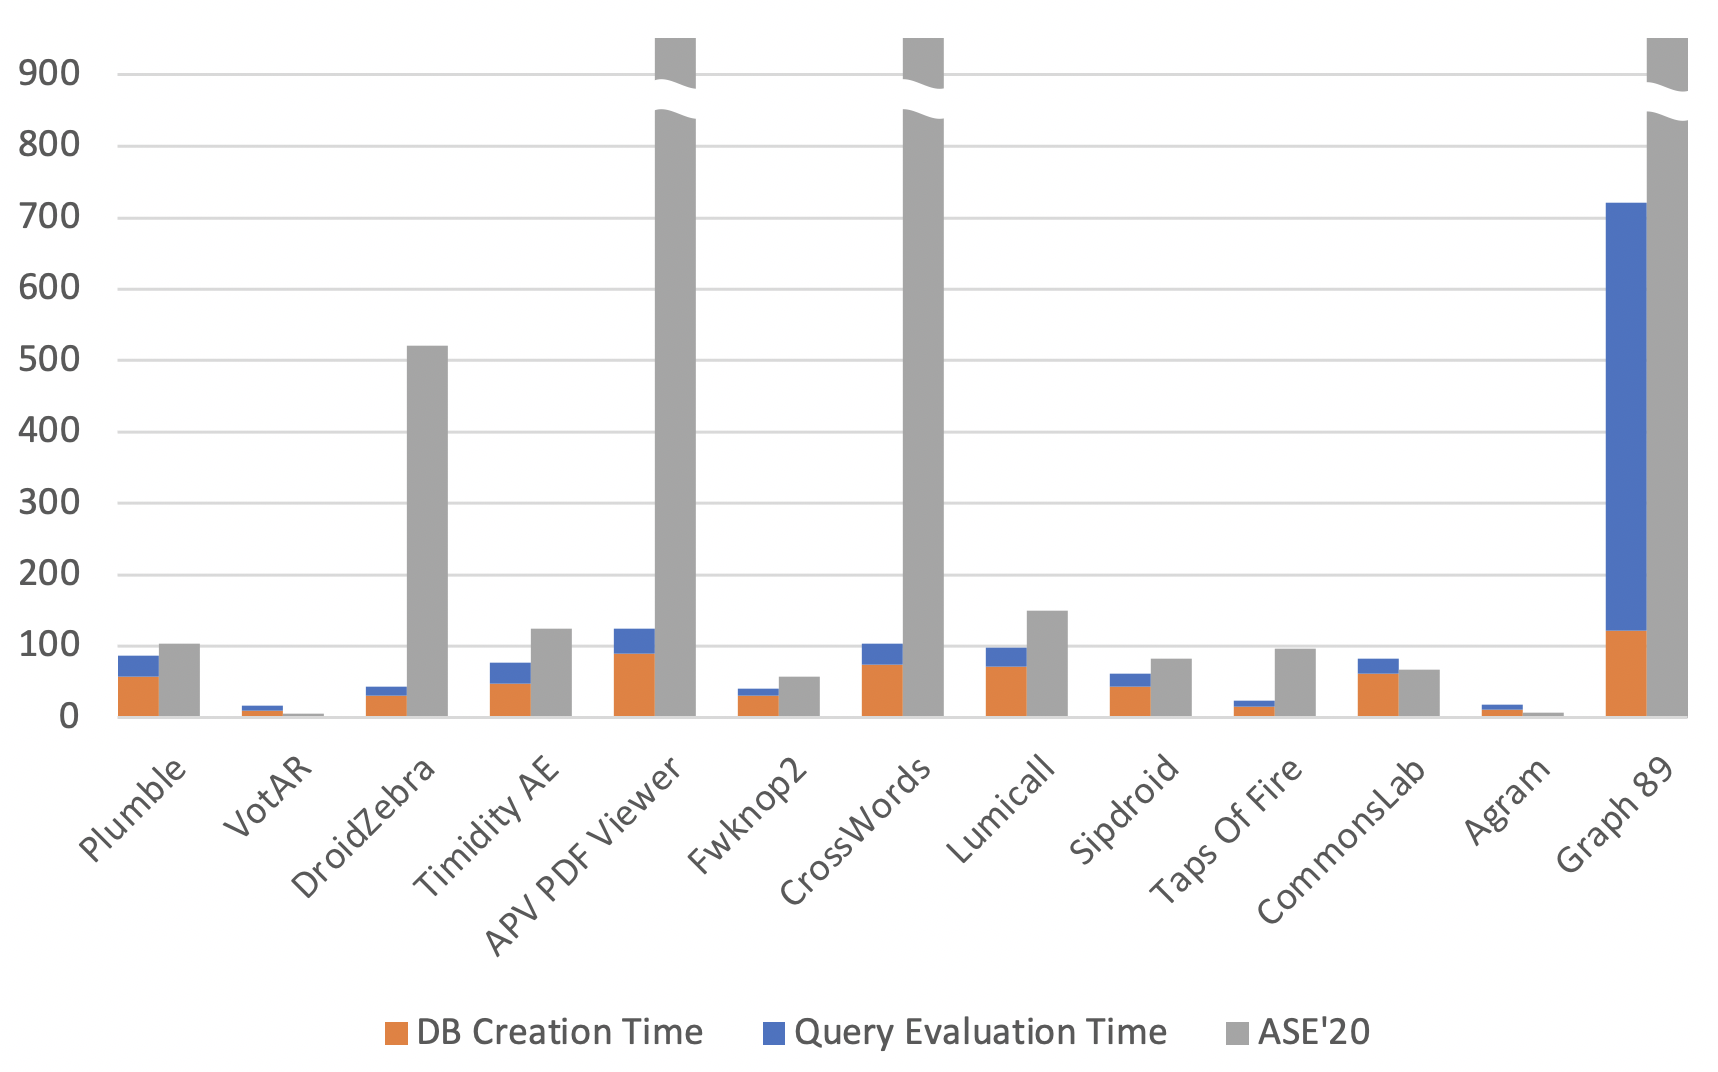
\includegraphics[width=0.48\textwidth]{img/graph}
  \vspace*{-1.5em}
  \caption{Analysis time of \ours and \lees}
  \label{fig:graph}
\vspace*{-.5em}
\end{figure}

\ours is scalable in that it can analyze large-scale programs. The analysis
time was 161.3 seconds on average for each app, including 103.8 seconds
for DB creation and 57.5 seconds for query processing.  DB creation
took more time than query processing except for {\it Graph 89}, and
the DB creation time was almost linear to the code size. \ours took
about 12 minutes at most to analyze {\it Tileless Map} having about one million
lines of code. Figure~\ref{fig:graph} shows the analysis time of \ours
compared to JN-Sum. \inred{describe the comparison result...}  Note
that once we create a database for a program, we can evaluate multiple queries on
it without re-creation to obtain various analysis results of the program.


\subsection{RQ3: Usefulness}
\begin{table}[t]
  \vspace{2mm}
  \caption{Bug detection results of real-world Android JNI apps}
  \label{table:RQ3}
  \vspace*{-1em}
  \centering
  \small
\renewcommand{\arraystretch}{.9}
  \begin{tabular}{l||r|r|r|r|r} 
    \multirow{4}{*}{\textbf{Application}} &
                                            \multicolumn{5}{c}{\textbf{Bug Kind}} \\\hhline{~||-----}
                                          & \multicolumn{2}{c|}{\textbf{Null}}   & \multicolumn{1}{c|}{\textbf{Missing}} & \multicolumn{1}{c|}{\textbf{Type}} & \multicolumn{1}{c}{\textbf{Wrong}} \\\hhline{~||~|~|~|~|~}
                                          & \multicolumn{2}{c|}{\textbf{Deref.}} & \multicolumn{1}{c|}{\textbf{Fun}} & \multicolumn{1}{c|}{\textbf{Mis.}} & \multicolumn{1}{c}{\textbf{\textbf{Sig.}}}  \\\hhline{~||-|-|-|-|-}
                                          & \multicolumn{1}{c|}{\textbf{\# TP}}   & \multicolumn{1}{c|}{\textbf{\# FP}} & \multicolumn{1}{c|}{\textbf{\# TP}} & \multicolumn{1}{c|}{\textbf{\# TP}} & \multicolumn{1}{c}{\textbf{\textbf{\# TP}}}  \\\hhline{=#=|=|=|=|=}

    APV PDF Viewer    & 0 & 1 & 0 & \cellcolor{\succcolor}2 & 0 \\ 
    CrossWords        & \cellcolor{\succcolor}3 & 1 & 0 & 0 & 0 \\ 
    Document Viewer   & 0 & 0 & 0 & \cellcolor{\succcolor}1 & 0 \\ 
    DroidZebra        & 0 & 1 & 0 & 0 & 0 \\ 
    FBReader          & 0 & 9 & 0 & \cellcolor{\succcolor}1 & 0 \\ 
    Graph 89          & \cellcolor{\succcolor}1 & 0 & 0 & \cellcolor{\succcolor}3 & 0 \\ 
    KeePassDroid      & \cellcolor{\succcolor}1 & 0 & 0 & 0 & 0 \\
    Lumicall          & 0 & 0 & \cellcolor{\succcolor}3 & 0 & 0 \\ 
    Lunary            & 0 & 1 & 0 & 0 & 0 \\
    Ministro          & 0 & 0 & 0 & \cellcolor{\succcolor}1 & 0 \\ 
    Navit             & 0 & 0 & 0 & \cellcolor{\succcolor}3 & 0 \\ 
    Hacker's Keyboard & 0 & 1 & 0 & 0 & 0 \\ 
    NetGuard          & 0 & 1 & 0 & 0 & 0 \\ 
    ObscuraCam        & 0 & 0 & \cellcolor{\succcolor}2 & 0 & 0 \\ 
    PrBoom            & 0 & 0 & 0 & 0 & \cellcolor{\succcolor}1 \\
    Sipdroid          & 0 & 0 & \cellcolor{\succcolor}4 & 0 & 0 \\ 
    Tileless Map      & 0 & 2 & 0 & \cellcolor{\succcolor}3 & 0 \\ 
    Tux Paint         & 0 & 4 & 0 & \cellcolor{\succcolor}3 & 0 \\ 
    VotAR             & 0 & 0 & 0 & 0 & \cellcolor{\succcolor}1 \\\hhline{=#=|=|=|=|=}
    \textbf{Total}    & 5 & 21 & 9 & 17 & 2 \\
  \end{tabular}
\end{table}

The bug checker of \ours detects four kinds of JNI interoperation bugs
that previous research~\cite{ILEA, LeeASE20} defined as follows:

\begin{itemize}
  \item {\it NullDereference}: dereferencing the {\tt null} value of Java in C
  \item {\it MissingFun}: calling a missing Java method from C
  \item {\it TypeMismatch}: declaring a C function with a different signature
    from its corresponding Java native method
  \item {\it WrongSignature}: calling a Java method using a method ID with a
    wrong signature in C
\end{itemize}


\begin{figure}[t]
  \centering
  \vspace{2mm}
  \begin{subfigure}[t]{0.5\textwidth}
    \begin{lstlisting}[style=java,xleftmargin=2.5em]
//EmulatorActivity.java
String tmp = null;
String folder = Util.GetInternalAppStorage(activity);

if (folder != null) {
  tmp = folder + "tmp";
  Util.CreateDirectory(tmp);
}
EmulatorActivity.nativeInitGraph89(..., tmp);
    \end{lstlisting}
    \begin{lstlisting}[style=cpp,xleftmargin=2.5em]
//wrappercommonjni.c
void nativeInitGraph89(..., jstring tmp_dir) {
   (*env)->GetStringUTFChars(env, tmp_dir, 0);
   ...
}
    \end{lstlisting}
    \vspace*{-.5em}
    \caption{NullDereference}
    \label{fig:bug1}
  \end{subfigure}
  \begin{subfigure}[t]{0.5\textwidth}
    \begin{lstlisting}[style=java,xleftmargin=2.5em]
//JpegRedaction.java
package org.witness.obscuracam.photo.jpegredaction;

public class JpegRedaction {
  private native void redactRegions(...);
  ...
}
    \end{lstlisting}
    \begin{lstlisting}[style=cpp,xleftmargin=2.5em]
//JpegRedaction.cpp
void
Java_org_witness_securesmartcam_jpegredaction_ JpegRedaction_redactRegions(...) {
  ...
}
    \end{lstlisting}
    \vspace*{-.5em}
    \caption{MissingFun}
    \label{fig:bug2}
  \end{subfigure}
  \begin{subfigure}[t]{0.5\textwidth}
    \begin{lstlisting}[style=java,xleftmargin=2.5em]
//MuPdfPage.java
private native static List<PageTextBox> search(...);
    \end{lstlisting}
    \begin{lstlisting}[style=cpp,xleftmargin=2.5em]
//mupdfdroidbridge.c
jobjectArray search(...){ ... }
    \end{lstlisting}
    \vspace*{-.5em}
    \caption{TypeMismatch}
    \label{fig:bug3}
  \end{subfigure}
  \begin{subfigure}[t]{0.5\textwidth}
    \begin{lstlisting}[style=java,xleftmargin=2.5em]
//PrBoomActivity.java
void OnMessage(String text);
void OnInfoMessage(String msg, int displayType);
    \end{lstlisting}
    \begin{lstlisting}[style=cpp,xleftmargin=2.5em]
//jni_doom.h
#define CB_CLASS_MSG_SIG  "(Ljava/lang/String;I)V"
#define CB_CLASS_INFMSG_SIG  "(Ljava/lang/String;I)V"

//jni_doom.c
mSendStr = (*env)->GetMethodID(env, jNativesCls,
                       "OnMessage", CB_CLASS_MSG_SIG);
    \end{lstlisting}
    \vspace*{-.5em}
    \caption{WrongSignature}
    \label{fig:bug3}
  \end{subfigure}
  \vspace*{-.5em}
  \caption{Four kinds of JNI interoperation bugs}
  \vspace*{-1em}
  \label{fig:bugs}
\end{figure}

Table~\ref{table:RQ3} summarizes the bug detection results of 19 out of 42
apps, on which \ours reported possible bugs.  The first
column shows app names, the second and the third columns show the
number of true and false positives for {\it NullDereference}, respectively, and
the fourth to six columns show the number of true positives for {\it
MissingFun}, {\it TypeMismatch}, and {\it WrongSig}, respectively.
\ours did not report any false positives for the last three bug kinds.
We confirmed true and false positives by manual inspection of the source code. 

\ours found 33 genuine bugs, but reported 21 false positives in 19 apps.
All false positives are reported only in the {\it NullDereference} bug
detection; \ours reported five true and 21 false alarms of {\it
NullDereference} in 11 apps, nine true alarms of {\it MissingFun} in
three apps, 17 true alarms of {\it TypeMismatch} in eight apps, and two true
alarms of {\it WrongSignature} in two apps. We manually checked that the false
positives come from diverse over-approximation issues of static analyses, but
one of the main causes is conditionally sanitized variables.  Many apps
have a code pattern that assigns a value to a variable only if the variable has
the {\tt null} value. Because our analysis does not support the
path-sensitivity that analyzes each execution path separately, it reports that
the variable may still have {\tt null} even after the conditional assignment.

Figure~\ref{fig:bugs} demonstrates four kinds of JNI interoperation bugs \ours
detected from real-world apps using simplified code.

Figure~\ref{fig:bugs}(a) shows a pattern in Graph 89 with the {\it NullDerefence} bug.
The Java code may call a C function {\tt nativeInitGraph89} with {\tt
null} as its last argument, because the variable {\tt tmp} has {\tt
null} when the method {\tt GetInternalAppStorage} returns {\tt null}.  The C
function calls a JNI function {\tt GetStringUTFChars} with the value as its
second argument, without checking whether it is {\tt null}. However, because the JNI
specification describes that the second argument of the functions must not be
{\tt null}~\cite{getstringutfchars}, the function may behave unexpectedly.
Note that calling JNI functions with wrong arguments may introduce various
unexpected behaviors, since JVMs do not validate the arguments because of
performance overhead~\cite{hwang2021justgen}.

\renewcommand{\texttt}[1]{%
  \begingroup
  \ttfamily
  \begingroup\lccode`~=`/\lowercase{\endgroup\def~}{/\discretionary{}{}{}}%
  \begingroup\lccode`~=`[\lowercase{\endgroup\def~}{[\discretionary{}{}{}}%
  \begingroup\lccode`~=`.\lowercase{\endgroup\def~}{.\discretionary{}{}{}}%
  \catcode`/=\active\catcode`[=\active\catcode`.=\active
  \scantokens{#1\noexpand}%
  \endgroup
}

Figure~\ref{fig:bugs}(b) shows a pattern in ObscuraCam with the {\it MissingFun} bug.
As described in Section~\ref{sec:merging}, JNI has a C function
naming convention for JVMs to link Java native methods to their corresponding C
functions. While a Java class {\tt JpegRedaction} declaring a native method
{\tt redactRegions} belongs to a package
\texttt{org.witness.obscuracam.photo.jpegredaction}, the corresponding C
function is named with a wrong package name
\texttt{org.witness.securesmartcam.jpegredaction}.  When calling the native
method, JVM fails to link it because of the wrongly named C function.


Figure~\ref{fig:bugs}(c) shows a pattern in Document Viewer with the {\it TypeMismatch} bug.
While the return type of a Java native method {\tt search}
is {\tt List<PageTextBox>}, the return type of the corresponding C function
{\tt search} is {\tt jobjectArray} corresponding to the Java built-in array
container. The return type mismatch has no effect on linking between
Java native methods and C functions. However, since it is an unspecified case in
the JNI specification, interoperations via such native methods may behave
differently on different JVMs~\cite{LeeASE20}. 


Figure~\ref{fig:bugs}(d) shows a pattern in PrBoom with the {\it WrongSignature} bug.
The C code tries to get an ID of a Java method {\tt OnMessage} with a
signature \texttt{(LJava/lang/String;I)V}, but the Java method has a different
signature \texttt{(LJava/lang/String;)V} taking a sole String argument. Because
the two signatures do not match, the C code always receives {\tt null}
instead of a method ID, and this example throws a Java exception. In
addition, it may introduce errors in subsequent instructions when using the
return value without null checking or calling JNI functions without handling the
thrown Java exception~\cite{jniexcept}.
